
\chapter{NB-IOT通信模块设计}
\section{模块总体介绍}

上海移远通信技术有限公司开发的bc35G通信模组支持 band8、band5、band20、band28频段,采用LCC贴片封装,尺寸为19.9mm*23.6mm*2.2mm,完全符合欧盟RoHs标准\cite{RoHs},外部参数如下:

\begin{table}[h!]
\caption{模块参数}
\begin{tabular}{ll}
\toprule
参数&说明\\
\midrule
供电&3.1V~4.2V,典型电压3.6V\\
省电&PSM模式下最大耗流 5uA\\
发射功率&23dBm +- 2dB\\
温度范围&正常工作温度: -35‘c~+75'C\\
\bottomrule
\end{tabular}
\label{模块参数}
\end{table}

模块的主要部分包括射频前端、电源管理、基带芯片。

射频前端主要包括功率放大器、滤波器,用于无线电信号和二进制信号的互相转换。

基带芯片则是用于信号处理,bc35G模块使用的是华为bionic系列芯片。


\section{供电}
电源是模块稳定运行的基础,对模块的性能以及使用寿命都有显著影响。同时由于NBIOT设备一般需要支持10年的正常使用,稳定可靠的电源也是重中之重。

锂亚电池电池由于其特殊的化学性质和钝化效应,储存寿命达到十年以上,被广泛运用与电子水表和电表等终端设备中作为电源,符合NBIOT应用的一般使用场景。同时其标称电压3.6V,与模块典型电压一致,所以锂亚电池
非常适合用于模块供电。

由于电源电压输出并不是理想直流输出,一般含有交流成分,比如惠州亿纬公司生产的AA型锂亚电池\cite{锂亚电池},在25°C的条件下,未放过电的电池在放电过程中每2分钟会释放一个150mA/0.1秒的脉冲,
所以在电源输入端并联了并联一个100uF的钽电容C1,以及100nF(C2)、100pF(C3)和22pF(C4)的滤波电容。

在模块开机或者电源接入时,一般会产生电涌,其对电子设备损害极大,所以为了避免电涌对模块的损害,在电源输入端增加一个TVS管(D1)以提高模块对浪涌电压的承受能力。

除了遵守一般的嵌入式模块电源设计要求,由于RF天线信号可能在电路中产生感应电流,所以通信模块的电源设计也要考虑到其与无线信号的相互干扰,简单的做法是在PCB布局上使VBAT电源线原理RF天线。

依据上述设计要求,输入端参考电路如图\ref{VBAT}。同时,根据模块的引脚定义表\ref{VBAT引脚定义},选用2脚和45脚作为电源输入的VBAT和GND。
\begin{figure}[H]
	\centering
	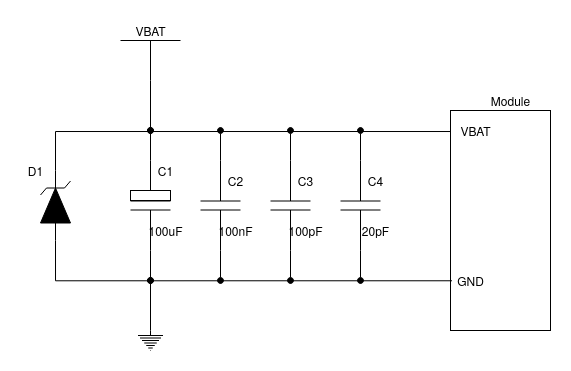
\includegraphics[width=10cm]{VBAT.png}
	\caption{VBAT}
	\label{VBAT}
\end{figure}

\begin{table}[h!]
\caption{VBAT引脚定义}
\begin{tabular}{lllll}
\toprule
  引脚名 & 引脚号 & 最小值 & 典型值 & 最大值\\
 \hline
 VBAT & 45,46 & 3.1V & 3.6V & 4.2V \\
 GND  & 2,43,47,48,51,52,54,59~66,71~74,81~83,92~94 & & 0 & \\
\bottomrule
\end{tabular}
\label{VBAT引脚定义}
\end{table}

\section{省电技术}

NBIOT技术的使用场景一般对设备不更换电源持续使用时间都有较苛刻的要求,比如10年的稳定工作。所以省电技术的支持就十分重要。

对于受限的物联网设备,省电技术一般有3种,分别是DRX(Discontinuous Reception),eDRX(extended DRX),PSM(Power Saving Mode),其基本思想是让通信设备终端周期性进入休眠模式,
在休眠期间不接受物理层消息,关闭收发的射频模块,从而达到省电目的。不同的省电技术一般可以通过不同的软件配置实现,在NBIOT物联网应用开发时,需要根据不同的使用场景使用不同的配置,使模
块能耗降到最低。

DRX技术是指一个周期内拥有两种工作状态,分别是激活态和休眠状态,仅在激活态时进行数据的接收、发送与处理,周期定时器一般可以通过核心网在设备入网时配置,一般配置为0.64s,1.28s,2.56s和
5.12s四种时间,当配置为0.64s时基本可以认为下行消息随时可以送达终端设备,实时性和延迟性能在三种技术中最好,但能耗消耗最大,所以一般用于对时延要求极高或者有稳定供电的场景,比如路灯的开关
应用。DRX模式的示意图如图\ref{drx模式}
\begin{figure}[H]
	\centering
	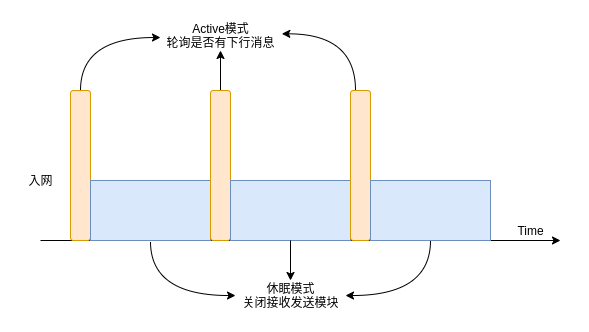
\includegraphics[width=10cm]{drx模式.png}
	\caption{drx模式}
	\label{drx模式}
\end{figure}

eDRX(扩展drx)技术在3GPP Release13中引入。一个eDRX周期相当与多个drx周期的组合,并且区分开接收下行消息和接收寻呼消息的周期。一个激活时间段和一个休眠时间段都
包含多个drx周期,并且激活周期和休眠周期各自包含一个PTW周期,激活周期中的PTW周期可以用于接收下行消息和寻呼消息,激活周期的PTW周期最大支持10.24s。休眠周期则不可以接受下行消息,只能接收寻呼消息,
休眠周期的PTW可以达到40分钟。在休眠周期是也可以通过寻呼消息唤醒终端设备从而接收下行消息,所以也可以认为消息可以时刻到达终端设备,由此可见eDRX技术对延时和能耗有一定的满足。eDRX模式的切换状态
如图\ref{eDRX模式}

\begin{figure}[H]
	\centering
	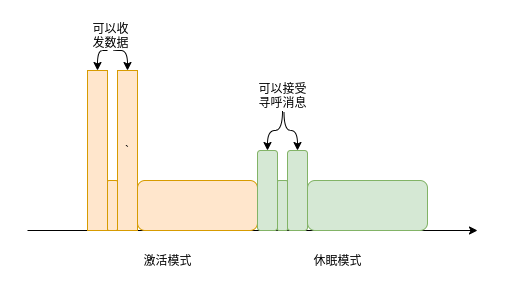
\includegraphics[width=10cm]{eDRX模式.png}
	\caption{eDRX模式}
	\label{eDRX模式}
\end{figure}

PSM模式则是对能耗有极致的要求,放弃了实时性,允许通信模块在PSM模式下完全不可达,所有耗电模块全部关闭。PSM模式的状态切换如图\ref{工作模式切换}。模块需要进入PSM模式,需要先通过 AT+PSM=1 开启模块PSM功能,
在模块入网或进行TAU操作时,将会请求进入PSM模式,得到核心网下发的T3324定时器数值,模块将会休眠直到T3324定时器过期或者模块主动发送消息,在休眠期间除了T3342时钟,所有模块都会关机。PSM模式如图\ref{PSM模式}

\begin{figure}[H]
	\centering
	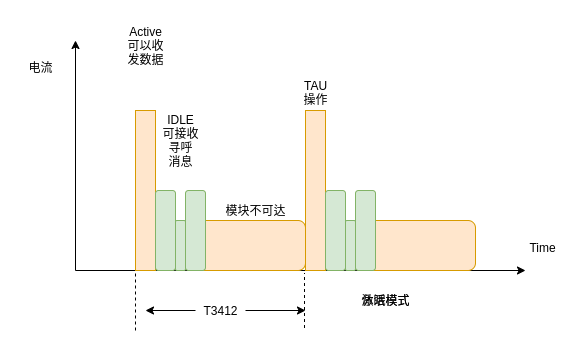
\includegraphics[width=10cm]{PSM模式.png}
	\caption{PSM模式}
	\label{PSM模式}
\end{figure}

模块在各种模式运行情况下,消耗电流如表\ref{消耗电流}

\begin{table}[h!]
\caption{消耗电流}
\begin{tabular}{llll}
\toprule
  模式 & 描述 & 典型值 & 最大值\\
 \hline
 PSM & 睡眠状态 & 3mA & 5mA \\
 IDLE  & 空闲状态 & 2mA & \\
 \multirow{3}{*}{Active} & 射频发射状态(23dBm)(B5/B8/B20) & 230mA & \\
 & 射频发射状态(23dBm)(B28) & 250mA & \\
 & 射频接收状态 & 61mA & \\
\bottomrule
\end{tabular}
\label{消耗电流}
\end{table}

\section{串口}
bc35g模块提供两对串口,分别为主串口和调试串口。主串口用于AT命令的通信、数据传输和固件升级,波特率为9600bps,在Active、Idle和PSM模式下均可工作,调试串口可以通过UE Log Viewer工具查看日志信息,波特率为921600bps。对于串口与上位机的连接,采用传统的DCE-DTE
(date terminal/control equivement)方式连接,模块作为DCE,连接方式如图\ref{DCT-DTE连接}

\begin{figure}[H]
	\centering
	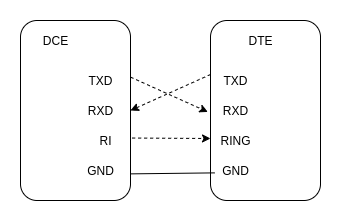
\includegraphics[width=10cm]{DCT-DTE连接.png}
	\caption{DCT-DTE连接}
	\label{DCT-DTE连接}
\end{figure}

RS232作为通用串行总线通信标准,在1970年有美国电子工业协会联合贝尔系统及一些终端生产厂家共同制定,用于DTE-DCE之间的通信,主要作用是将MCU输出的TTL电平转换成RS232电平。TTL电平是指在输出电路上电压大于等于2.4V为逻辑1,电压小于0.4V为逻辑
0,而在输入电路上,电压大于等于2.0v为逻辑1,电压小于等于0.8V为逻辑0。而RS232电平规定-15V 到 -3V代表逻辑1,+3V 到 +15V代表逻辑0。为了使模块能够接入PC调试,需要在MCU引出的串口引脚与PC连接之间加上RS232电平
转换芯片,并且为了降低串口功耗,在电路中加入1k欧姆电阻降低串口电流,RS232转换电路如图\ref{RS232连接图}

\begin{figure}[H]
	\centering
	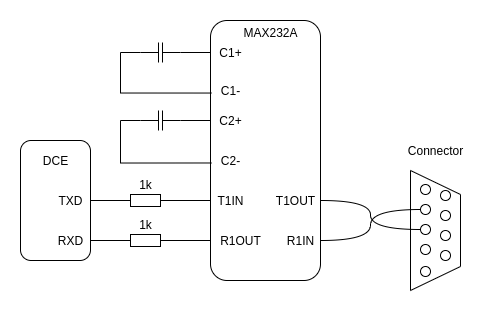
\includegraphics[width=10cm]{RS232连接图.png}
	\caption{RS232连接图}
	\label{RS232连接图}
\end{figure}

\section{射频天线}
BC35G天线部分预留了pi型匹配电路如图\ref{ANT},以便对天线性能调节。C1和C2两个电容将大多数交流成分滤除,R1为0欧电阻,充当pi型RC滤波电路的电感。为了确保射频信号的性能以及可靠性,需要遵循pi型匹配电路的layout。既要保证电容电感布局靠近,也要防止出现stub\cite{OKgagaga,stubeffect}
\begin{figure}[H]
	\centering
	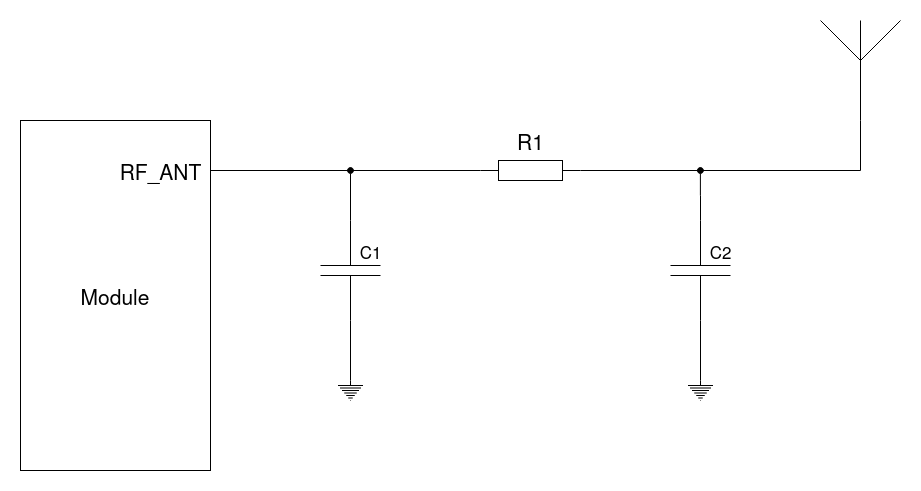
\includegraphics[width=10cm]{ANT.png}
	\caption{ANT}
	\label{ANT}
\end{figure}

对于模块的射频信号线,需要保证PCB上所有射频信号线的特性阻抗控制在50欧姆,控制射频信号新特性阻抗一般采取微带线和共面波导的设计方式,通过控制射频信号线材料的介电常数,地平面参考高度(H),离地间隙(S)以及走线宽度(W),从而改变射频信号线的特性阻抗。

微带线是指在介质基片上由单一的导体带构成的微波传输线,其特点是体积小、重量轻、可用频段宽、可靠性高、制造成本低,但损耗比较大,功率范围比较窄,微带线的结构示意图如图\ref{微带线}

\begin{figure}[H]
	\centering
	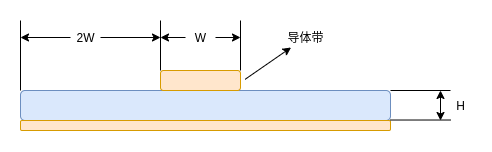
\includegraphics[width=10cm]{微带线.png}
	\caption{微带线}
	\label{微带线}
\end{figure}

共面波导是指在一个面上由两个导体平面夹着一个中心导体带的结构,其相比于微带线,具有工艺简单、屏蔽性能好,接地电感低等优点,但是其衰减损耗更大,导热能力也不理想,导致不适用于大功率的放大器。两层共面波导的结构示意图如\ref{共面波导}

\begin{figure}[H]
	\centering
	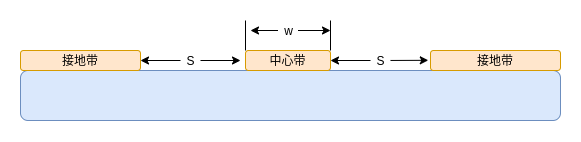
\includegraphics[width=10cm]{共面波导.png}
	\caption{共面波导}
	\label{共面波导}
\end{figure}

在实际的电路设计中,为了确保射频信号的性能和可靠性能够满足要求,在电路模拟时需要精确地控制射频信号线的阻抗为50欧姆,射频引脚到天线连接器之间的走线避免走90度角,情况允许尽量走135度角。与射频引脚相连的GND引脚也不做热焊盘,要与地充分接触。

\section{USIM卡座}
USIM全称为Universal Subscriber Identity Module,是SIM卡(Subscriber Identity Module)的升级。USIM卡是一个内置有MCU的芯片卡,内部包含一个
位CPU,一个3到8kbit的程序存储器(ROM),一个6到16kbit的工作存储器(RAM),一个128到256kbit的数据存储器(EEPROM)和串行通信单元5个模块,需要5个引脚才能正常工作,
分别是电源VDD,时钟CLK,数据IO Data,复位 RST,接地 GND,引脚的定义及功能如表\ref{USIM引脚定义}

\begin{table}[h!]
\caption{USIM引脚定义}
\begin{tabular}{lll}
\toprule
  引脚名称 & 引脚号 & 描述 \\
 USIM\_VDD & 38 & 外部USIM卡供电电源,电压3.0v \\
 USIM\_CLK  & 41  & 外部USIM卡时钟线  \\
 USIM\_DATA & 40 & 外部USIM卡数据线  \\
 USIM\_RST & 39 &  外部USIM卡复位线  \\
 USIM\_GND & 42 & 外部USIM卡转用地  \\
\bottomrule
\end{tabular}
\label{USIM引脚定义}
\end{table}

支持3GPP规范功能的USIM卡使模块能够接入运营商网络,USIM功能包括模块和卡座,为了确保USIM卡的性能以及避免与射频、电源模块的干扰,须遵循以下设计原则:

\begin{enumerate}
\item USIM卡座和模块尽量靠近摆放,尽量保证USIM信号线布线长度不超过200mm保证信号品质
\item 外部USIM信号线布线应尽量远离射频线号线走线及电源VBAT走线
\item 防止USIM\_DATA和USIM\_CLK信号干扰,两线之间加入地屏蔽,并保持一定的距离。在USIM\_RST信号也需要地保护
\item USIM\_DATA, USIM\_VDD, USIM\_CLK, 和USIM\_RST并联33pF电容滤除射频线号线的的干扰
\item 为了防止静电,在卡座和模块之间增加TVS管,TVS管的寄生电容应不大于55pF
\end{enumerate}


USIM卡座电路图如\ref{USIM}
\begin{figure}[H]
	\centering
	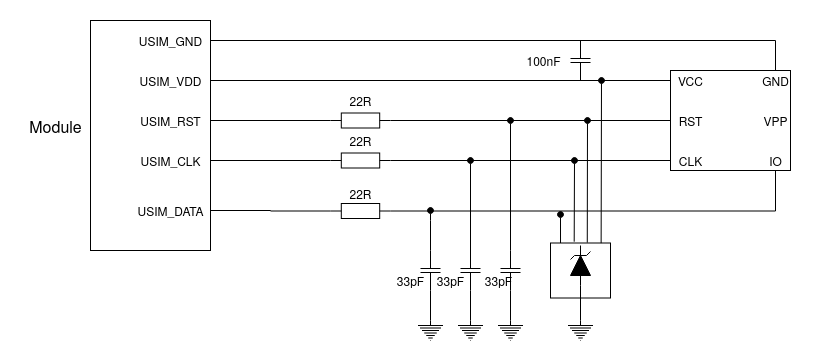
\includegraphics[width=10cm]{USIM.png}
	\caption{USIM}
	\label{USIM}
\end{figure}

\section{本章小结}

本章讨论了BC35G模块的外围电路设计,包括USIM卡座、电源、天线以及串口,主要关注于各部分之间的信号干扰避免,通过合理使用滤波电容,不同部分在电路板上的位置的相对远离,以达到良好的射频信号性能以及可靠性。同时通过TVS管等方式降低电涌对设备的损害。